\documentclass[border=15pt, multi, tikz]{standalone}
\usepackage{import}
\subimport{../../layers/}{init}
\usetikzlibrary{positioning}
\usetikzlibrary{3d} %for including external image 

\def\ConvColor{rgb:yellow,5;red,2.5;white,5}
\def\ConvReluColor{rgb:yellow,5;red,5;white,5}
\def\PoolColor{rgb:red,1;black,0.3}
\def\DcnvColor{rgb:blue,5;green,2.5;white,5}
\def\SoftmaxColor{rgb:magenta,5;black,7}
\def\SumColor{rgb:blue,5;green,15}

\begin{document}
\begin{tikzpicture}
\tikzstyle{connection}=[ultra thick,every node/.style={sloped,allow upside down},draw=\edgecolor,opacity=0.7]
%%%%%%%%%%%%%%%%%%%%%%%%%%%%%%%%%%%%%%%%%%%%%%%%%%%%%%%%%%%%%%%%%%%%%%%%%%%%%%%%%%%%%%%%
%% Draw Layer Blocks
%%%%%%%%%%%%%%%%%%%%%%%%%%%%%%%%%%%%%%%%%%%%%%%%%%%%%%%%%%%%%%%%%%%%%%%%%%%%%%%%%%%%%%%%
\node[canvas is zy plane at x=0] (temp) at (-3,0,0) {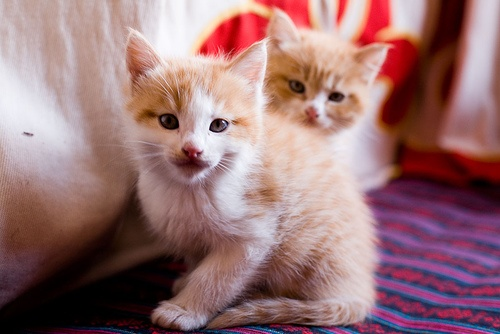
\includegraphics[width=8cm,height=8cm]{cats.jpg}};
% conv1_1,conv1_2,%pool1
\pic[shift={(0,0,0)}] at (0,0,0) {RightBandedBox={name=cr1,caption=conv1,%
        xlabel={{"64","64"}},zlabel=I,fill=\ConvColor,bandfill=\ConvReluColor,%
        height=40,width={2,2},depth=40}};
\pic[shift={(0,0,0)}] at (cr1-east) {Box={name=p1,%
        fill=\PoolColor,opacity=0.5,height=35,width=1,depth=35}};
% conv2_1,conv2_2,pool2
\pic[shift={(2,0,0)}] at (p1-east) {RightBandedBox={name=cr2,caption=conv2,%
        xlabel={{"64","64"}},zlabel=I/2,fill=\ConvColor,bandfill=\ConvReluColor,%
        height=35,width={3,3},depth=35}};
\pic[shift={(0,0,0)}] at (cr2-east) {Box={name=p2,%
        fill=\PoolColor,opacity=0.5,height=30,width=1,depth=30}};
% conv3_1,conv3_2,pool3
\pic[shift={(2,0,0)}] at (p2-east) {RightBandedBox={name=cr3,caption=conv3,%
        xlabel={{"256","256","256"}},zlabel=I/4,fill=\ConvColor,bandfill=\ConvReluColor,%
        height=30,width={4,4,4},depth=30}};
\pic[shift={(0,0,0)}] at (cr3-east) {Box={name=p3,%
        fill=\PoolColor,opacity=0.5,height=23,width=1,depth=23}};
% conv4_1,conv4_2,conv4_3,pool4
\pic[shift={(1.8,0,0)}] at (p3-east) {RightBandedBox={name=cr4,caption=conv4,%
        xlabel={{"512","512","512"}},zlabel=I/8,fill=\ConvColor,bandfill=\ConvReluColor,%
        height=23,width={7,7,7},depth=23}};
\pic[shift={(0,0,0)}] at (cr4-east) {Box={name=p4,%
        fill=\PoolColor,opacity=0.5,height=15,width=1,depth=15}};
% conv5_1,conv5_2,conv5_3,pool5
\pic[shift={(1.5,0,0)}] at (p4-east) {RightBandedBox={name=cr5,caption=conv5,%
        xlabel={{"512","512","512"}},zlabel=I/16,fill=\ConvColor,bandfill=\ConvReluColor,%
        height=15,width={7,7,7},depth=15}};
\pic[shift={(0,0,0)}] at (cr5-east) {Box={name=p5,%
        fill=\PoolColor,opacity=0.5,height=10,width=1,depth=10}};    
%% fc6, fc7 -> cr6, cr7
\pic[shift={(1,0,0)}] at (p5-east) {RightBandedBox={name=cr6_7,caption=fc to conv,%
        xlabel={{"4096","4096"}},fill=\ConvColor,bandfill=\ConvReluColor,%
        height=10,width={10,10},depth=10}};  
%% fc8 -> cr8 (score32)
\pic[shift={(1,0,0)}] at (cr6_7-east) {Box={name=score32,caption=fc8 to conv,%
        xlabel={{"K","dummy"}},fill=\ConvColor,%
        height=10,width=2,depth=10,zlabel=I/32}};
%%%%%%%%%%%%%%%%%%%%%%%%%%%%%%%%%%%%%%%%%%%%%%%%%%%%%%%%%%%%%%%%%%%%%%%%%%%%%%%%%%%%%%%%
%%Joining with previous streams (fcn-16s)
%% Upsampling Deconv Layer
%% Dcnv32    
\pic[shift={(1.5,0,0)}] at (score32-east) {Box={name=d32,%
        xlabel={{"K","dummy"}},fill=\DcnvColor,%
        height=15,width=2,depth=15,zlabel=I/16}};  
%% score16
\pic[shift={(0,-4,0)}] at (d32-west) {Box={name=score16,%
            xlabel={{"K","dummy"}},fill=\ConvColor,%
            height=15,width=2,depth=15,zlabel=I/16}};
%% Elementwise sum between score16 and up32
\pic[shift={(1.5,0,0)}] at (d32-east) {Ball={name=elt1,%
        fill=\SumColor,opacity=0.6,%
        radius=2.5,logo=$+$}};
%%%%%%%%%%%%%%%%%%%%%%%%%%%%%%%%%%%%%%%%%%%%%%%%%%%%%%%%%%%%%%%%%%%%%%%%%%%%%%%%%%%%%%%%
%%Joining with previous streams (fcn-8s)
%% Upsampling Deconv Layer
%% Dcnv16    
\pic[shift={(1.5,0,0)}] at (elt1-east) {Box={name=d16,%
        xlabel={{"K","dummy"}},fill=\DcnvColor,%
        height=23,width=2,depth=23,zlabel=I/8}};  
%% score8
\pic[shift={(0,-6,0)}] at (d16-west) {Box={name=score8,%
        xlabel={{"K","dummy"}},fill=\ConvColor,%
        height=23,width=2,depth=23,zlabel=I/8}};
%% Elementwise sum between score16 and up32
\pic[shift={(1.5,0,0)}] at (d16-east) {Ball={name=elt2,%
        fill=\SumColor,opacity=0.6,%
        radius=2.5,logo=$+$}};
%%%%%%%%%%%%%%%%%%%%%%%%%%%%%%%%%%%%%%%%%%%%%%%%%%%%%%%%%%%%%%%%%%%%%%%%%%%%%%%%%%%%%%%%%    
%%% Output
%%%%%%%%%%   
%% Dcnv8    
\pic[shift={(2.5,0,0)}] at (elt2-east) {Box={name=d8,%
        xlabel={{"K","dummy"}},fill=\DcnvColor,%
        height=40,width=2,depth=40}}; 
%%%%%%%%%%   
%% softmax    
\pic[shift={(1,0,0)}] at (d8-east) {Box={name=softmax,caption=softmax,%
        xlabel={{"K","dummy"}},fill=\SoftmaxColor,%
        height=40,width=2,depth=40,zlabel=I}}; 
%%%%%%%%%%%%%%%%%%%%%%%%%%%%%%%%%%%%%%%%%%%%%%%%%%%%%%%%%%%%%%%%%%%%%%%%%%%%%%%%%%%%%%%%
%% Draw connections
%%%%%%%%%%%%%%%%%%%%%%%%%%%%%%%%%%%%%%%%%%%%%%%%%%%%%%%%%%%%%%%%%%%%%%%%%%%%%%%%%%%%%%%%
\draw [connection]  (p1-east)    -- node {\midarrow} (cr2-west);
\draw [connection]  (p2-east)    -- node {\midarrow} (cr3-west);
\draw [connection]  (p3-east)    -- node {\midarrow} (cr4-west);
\draw [connection]  (p4-east)    -- node {\midarrow} (cr5-west);
\draw [connection]  (p5-east)    -- node {\midarrow} (cr6_7-west);
\draw [connection]  (cr6_7-east)   -- node {\midarrow} (score32-west);
\draw [connection]  (score32-east) -- node {\midarrow} (d32-west);

\path (p4-east) -- (cr5-west) coordinate[pos=0.25] (between4_5) ;
\draw [connection]  (between4_5)    -- node {\midarrow} (score16-west-|between4_5) -- node {\midarrow} (score16-west);
\draw [connection]  (d32-east) -- node {\midarrow} (elt1-west);
\draw [connection]  (score16-east) -- node {\midarrow} (score16-east -| elt1-south) -- node {\midarrow} (elt1-south);
\draw [connection]  (elt1-east) -- node {\midarrow} (d16-west);

\path (p3-east) -- (cr4-west) coordinate[pos=0.25] (between3_4) ;
\draw [connection]  (between3_4) -- node {\midarrow} (score8-west-|between3_4) -- node {\midarrow} (score8-west);
\draw [connection]  (d16-east) -- node {\midarrow} (elt2-west);
\draw [connection]  (score8-east) -- node {\midarrow} (score8-east -| elt2-south)-- node {\midarrow} (elt2-south);
\draw [connection]  (elt2-east) -- node {\midarrow} (d8-west);
\draw [connection] (d8-east) -- node{\midarrow} (softmax-west);
%%%%%%%%%%%%%%%%%%%%%%%%%%%%%%%%%%%%%%%%%%%%%%%%%%%%%%%%%%%%%%%%%%%%%%%%%%%%%%%%%%%%%%%%

\end{tikzpicture}
\end{document}\grid
